\documentclass[a4paper]{article} %indique la classe du document, et les options 

%le pr�ambule
\usepackage{graphicx}	% Including figure files

%\title{Protoplanetary physical model used as input for Nautilus}   

\title{\bf Disk physical model for Nautilus}   




        % Les param̬tres du titre� : titre, auteur, date
\author{V. Wakelam, L. Majumdar}
\date{Feb 2017}                       % La date n'est pas requise (la date du
                              % jour de compilation est utilis̩e en son
			      % absence)

\sloppy                       % Ne pas faire d̩border les lignes dans la marge

\begin{document}

\maketitle                    % Faire un titre utilisant les donn̩es
                              % pass̩es �  \title, \author et \date

%\section{abstract}
We present the physical model used as input for Nautilus. The temperature, density and visual extinction profiles are computed in the vertical direction at a specific radius from the central star. The dust temperature can also be provided. To mimic the grain sedimentation and growth, the abundance of grains, size and AV/NH conversion factor can be given for each altitude. This code computes these quantities from some specific parameters. A fortran procedure has been created to produce a file containing all these quantities at each height, starting from the most external point of the envelop. This document shows the exact calculations that are being done. For more physical description, we refer to Hersant et al. (2009); Wakelam et al. (2016).
%\end{abstract}

\section{Input parameters}

The input parameters for the IDL procedure are the following:\\
\begin{itemize}

\item[-] Number of spatial points in the vertical direction (resolution of the grid): nbpoints.

\item[-] Radius in disk from the star where we want the vertical structure in AU: r.

\item[-] Mass of the central object in g: M$_*$.

\item[-] Mid-plane temperature (in K) of the gas at radius (R) in AU constrained by the observations: T$_{\rm midplan R}$.

\item[-] Gas temperature (in K) in the atmospheric limit (at 4 scale height) at radius (R) constrained by the observations : T$_{\rm atmos R}$.

\item[-] Surface density at R AU (in g.cm$^{-2}$): $\Sigma_{R}$. This is constrained by observations. 

\item[-] UV irradiation field coming from the central star at R AU: UV$_{R}$. In our model, we assume that the UV spectrum of the central star has the same 
as the ISM. Thus this parameter is a factor of Draine's ISM UV field.

\item[-] Exponent of the radial variation of temperature: q. This parameter is constrained by observations. 

\item[-] Stiffness of the vertical temperature profile: $\sigma$.

\item[-] Exponent of the radial variation of density: d. This is constrained by observations. 

\item[-] Dust to gas mass ratio: dtogm$\_$up. This is usually taken to $10^{-2}$. In the case of homogeneous grains, this value is used for all altitudes. In the case of sedimentation, this parameter is the dust to gas mass ratio in the upper part of the disk.

\item[-] Grain sizes (in cm): small$\_$grains and big$\_$grains. We assume that the small grains are in the upper atmosphere while the big grains are in the lower atmosphere. 

\item[-] Transition altitude (in z/H): transition$\_$altitude. This is the altitude of transition of small grains to big grains.
\end{itemize}

\section{Constants}

Here are the constants that are used for the calculation:\\
\begin{itemize}
\item[-] Boltzmann constant: $k_B$ = 1.38054$\times 10^{-16}$ in erg.K$^{-1}$.

\item[-] Conversion factor from AU to cm: autocm=1.49597$\times 10^{13}$. 

\item[-] Mean molecular weight of the gas: $\mu$=2.4. The mean molecular weight of the gas is by default equal
to the solar metallicity value $\mu$=2.4 but can be varied between $\mu$=2 (pure molecular hydrogen) and $\mu$=3 (highly metal rich). See Mayer et al. (2008) for more discussions.

\item[-] Atomic mass unit: amu=1.66043$\times 10^{-24}$ g 

\item[-] Gravitational constant: G=6.668$\times 10^{-8}$ cm$^3$g$^{-1}$s$^{-2}$

\item[-] Conversion factor of H column density to Av: $AV/NH_0$ = 6.25$\times 10^{-22}$. From Wagenblast \& Hartquist (1989). 

\end{itemize}

\section{Computation of mid-plane and atmospheric temperatures at a given radius r}

 If the mid-plane and atmospheric temperatures are observationally constrained at R AU, then mid-plane and atmospheric temperatures at the selected radius r are computed through:


\begin{equation}
\rm T_{midplan } = T_{midplan R} \times \Big(\frac{r}{R}\Big)^{-q}
\end{equation}
\begin{equation}
\rm T_{atmos } = T_{atmos R} \times  \Big(\frac{r}{R}\Big)^{-q}
\end{equation}
\\
%In some conditions, it is not the temperature at 100 AU that are given so the user should change this according to what they have. The mid-plan temperature for instance may be the same for several radii.

\section{Computation of the scale heights H and H$_{atmos}$}

H is the scale height (in cm) defined by the mid-plane temperature and assuming vertical static equilibrium. H is computed by the equation:\\
\begin{equation}
\rm H = \sqrt{\frac{k_B \times T_{mid-plan} \times (r \times autocm)^3}{\mu amu G M_*}} 
\end{equation}
\\
H$_{atmos}$ is the scale height defined by T$_{atmos}$:\\
\begin{equation}
\rm H_{atmos} = \sqrt{\frac{k_B  T_{atmos} \times (r  autocm)^3}{\mu amu G M_*}} 
\end{equation}

\section{Computation of the vertical grid}

The total size of the box is 4H. z will be a table of spatial points vertically distributed and equally spaced. z is computed with the formula given by Franck Hersant:\\
for i=0,nbpoints-1 do $\rm z(i) = (1-\frac{2\times i}{2\times nbpoints-1}) \times 4H$\\

\section{Computation of the 1D vertical temperature profile}

We are using the definition by Williams \& Best (2014) meaning that T is constant above 4H. 
Below this height, the temperature is computed using a sinus:\\
\begin{equation}
	\rm Tz(i) = T_{midplan} + (T_{atmos} - T_{midplan}) \times \Big(\sin{\Big(\frac{\pi z(i)}{2z(0)}\Big)}\Big)^{2\sigma}
\end{equation}

\section{Computation of the 1D vertical density profile}

The density is computed assuming the hydrostatic equilibrium.
\\
We first compute: $\Omega = \frac{G\times M_*}{(r\times au-conv)^3}$.\\
\\
We compute the maximum H$_2$ density (in cm$^{-3}$), i.e. the density in the mid-plane from the surface density. 
\begin{equation}
\rm nzH2_{midplan} = \Sigma_{R} \times \Big(\frac{r}{R}\Big)^{-d}\times \frac{1}{\mu amu H \sqrt{2\pi}}
\end{equation}
\\
The most external point of the atmosphere nzH2$_{0}$ will have a density of 1 for the moment.\\
\\
We then compute the H$_2$ density (in cm$^{-3}$) for each z point:\\
\begin{equation}
\rm int(i) = int(i-1) - (\ln{Tz(i)} - \ln{Tz(i-1)}) - \frac{\Omega \mu  amu}{k_B Tz(i) z(i) (z(i)-z(i-1))}
\end{equation}
\begin{equation}
\rm 	nzH2(i) = \exp{(int)}
\end{equation}
\\
Then a rescaling of the density is done so that the maximum density of the distribution is nzH2$_{midplan}$:\\
for i=0,nbpoints-1 do nzH2(i) = $\frac{nzH2(i)}{max(nzH2)\times nzH2_{midplan}}$

\section{Computation of the 1D vertical visual extinction profile}
	
In the previous version of the code, we would compute the H column density above 4H (the most external point of our grid) assuming an ercf to the gaussian 
distribution above that point:\\
\begin{equation}
\rm int=\frac{4H}{\sqrt{2} \times H_{atmos}}
\end{equation}
\begin{equation}
\rm NH(0) = 2\times \frac{nzH2(0)\times H_{atmos}\times \sqrt{2}\times \exp{(-int^2)}}{int+\sqrt{int^2+2}}
\end{equation}
The factor of 2 is to take into account the fact that we compute total H column density from H2 densities. There is here an approximation since at this altitude, part of hydrogen will be atomic.\\
This formula was however wrong (the density should not be nzH2(0) and a $\pi$ was missing. Thus we have decided to assume a null NH(0). After some tests, we have found that it did not make any difference except for the first point. This has no impact on the model and it simplifies the calculation.
\\
From NH(0), we compute Avz(0):\\
\begin{equation}
\rm Avz(0) = NH(0)\times AV/NH_0\times \frac{dtogm}{10^{-2}} \times \frac{10^{-5}}{r_{grain}}
\end{equation}
So Avz(0) = 0.\\
Computation of Avz for other points:\\
for i=1,nbpoints-1 do 
\begin{equation}
\rm Avz(i) = Avz(i-1) + 2\times nH2z(i)\times (z(i-1)-z(i)) \times AV/NH_0\times \frac{dtogm}{10^{-2}} \times \frac{10^{-5}}{r_{grain}}
\end{equation}
with $r_{grain}$ the grain radius (in cm). This is to change the Av according to the radius of the grains while changing it.
	
\section{Computation of the UV irradiation factor}

We also compute the UV irradiation factor at the requested radius.
The initial UV is divided by two because since we do not make a full 3D 
 transfer, we assume that only half of the photons irradiated from the star 
 diffuse into the disk, the other half diffuse in the opposite direction.
 The UV flux coming from the star is assumed to have the same 
 spectrum as the interstellar DRAINE field multiplied by a certain amount and diluted as 1/r$^2$.
\begin{equation}
\rm UVfactor = \frac{UVR}{2\times \sqrt{(r/R)^2+(4H/(R\times au-conv)^2)}}
\end{equation}

\section{Calculation of the total surface density at radius R}

The total surface density $\Sigma$ depends on the total mass of the disk and the outer radius. The mass of the disk is:
\begin{equation}
\rm M = \int_0^\infty 2\pi \times r \times \Sigma(r) dr
\end{equation}
If d is 1.5, the final total surface density at R AU is:
\begin{equation}
\Sigma_{R} = \frac{M\times (R )^{-1.5} \times 0.5}{2\times \pi \times (r_{out})^{0.5}}
\end{equation} 

%\section{Parameter values used for modeling}
%
%\begin{itemize}
%
%\item [-] The number of grid points is usually nbpoints = 64. This value is based on previous tests and checks.\\
%
%\item[-] The exponent of the radial variation of temperature q and of density d are usually taken to be 0.5 and -1.5 respectively based on angularly resolved CO interferometric analysis performed by Pi�tu et al. (2007). \\
%
%\item[-] The stiffness of the vertical temperature profile is taken to be 2 but seems to be a rather free parameter.\\
%
%\item[-] The other parameters depends on the source and are given in Table~\ref{source_param}.\\
%
%\item [-] Disk masses are from Guilloteau et al. (2011). 
%\end{itemize}

\begin{table*}
\caption{List of parameters used for our disk models}
\centering
\begin{tabular}{c|c|c|c|c|c}
 \hline
 & LkCa15$^a$ & DMTAU$^b$ & MWC 480$^c$  &  GG Tau$^d$ & TW Hya$^e$ \\
 \hline
 
 
 R (AU)    &   100  &  100   &  100   &  200    & 10    \\

 
UV Flux & 2550 & 410 & 8500  &  1500$^f$  & 3400 \\
 
 Age (Myr) & 3-5  & 5 & 7  & 1-5    & 3-10 \\
 
 Stellar Mass (g) & $2\times 10^{33}$ & $1.054\times 10^{33}$ & $3.640\times 10^{33}$    &   $2.53\times 10^{33}$   &  $0.80\times 10^{33}$   \\
 
 T$_{\rm midplan R}$ (K) & 15 & 15 & 30   & 14 & 20 \\
 
 T$_{\rm atmos R}$ (K) & 20 & 30 & 48  &  30 & 104   \\
 
 Disk mass (solar mass) & 0.03 & 0.03 & 0.18    & 0.12   & 0.06 \\
 
 r$_{out}$ (AU) & 550 & 800 & 500   &  800   & 172 \\
 
 Total surface density at R (g.cm$^{-2}$) & 0.9 & 0.75 & 5.7   & 14.9  & 0.79 \\
 
 Temperature exponent (q)    &   0.5  &   0.5  & 0.5   &  1.1    &  0.55   \\

Density exponent (d)   & 1.5    &  1.5   &   1.5  & 2.75     &   1.5 \\

Temperature Stiffness ($\sigma$)  & 2    &  2   &   2  & 2     &   2 \\
 \hline
  \multicolumn{6}{l}{\scriptsize Notes: a-b-c: Guilloteau et al. (2011); Pitu et al. (2007); Bergin et al. (2004); Guilloteau \& Dutrey (1998)}\\
  
 \multicolumn{6}{l}{\scriptsize  d: Guilloteau et al. (1999); Dutrey et al. (2014)}\\
 
 \multicolumn{6}{l}{\scriptsize  e: Andrews et al. (2012); Herczeg et al. (2004), Qi et al. (2006)}\\

 \multicolumn{6}{l}{\scriptsize f. No measurement. Other canonical values could be used as well: 500, 3000 by discussing with A. Dutrey}\\
  
  
  
  
  
  \end{tabular}
\label{source_param}
\end{table*}


\section{Typical results}\label{results}

We here show results for the following parameters (for DMTAU):
\begin{itemize}
\item[-] r = 300 AU, 
\item[-] M$_*$ =  $1.054\times 10^{33}$ g, 
\item[-] T$_{midplan, 100}$ = 15 K,
\item[-] T$_{midplan, 100}$ = 30 K,
\item[-] UV100AU = 410,                 
\item[-] q = 0.5,                    
\item[-] $\sigma$ = 2,            
\item[-] $\Sigma_{100}$ = 0.8 g.cm$^{-2}$,    
\item[-] d = 1.5,  
\item[-] dtogm = $10^{-2}$                 
\end{itemize}

\begin{figure}
\centering
 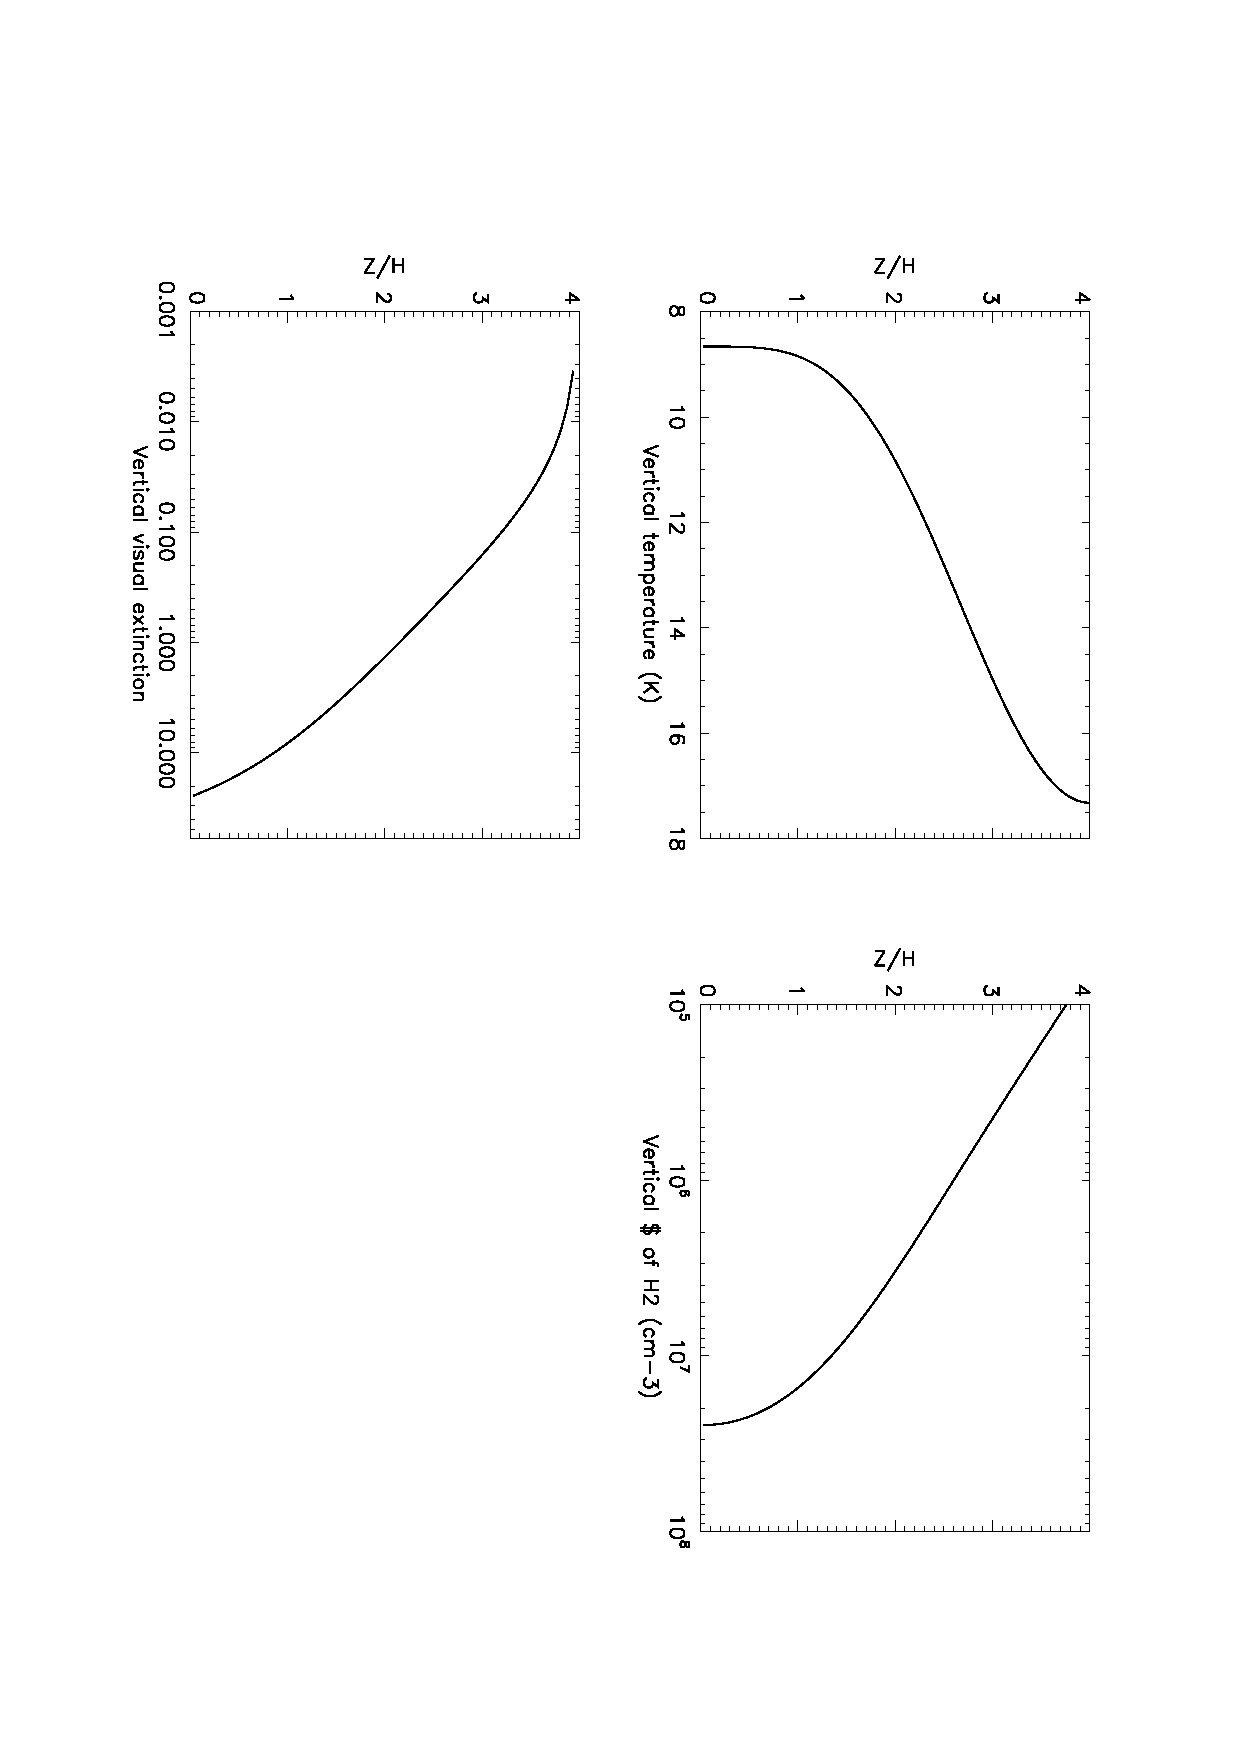
\includegraphics[angle=90,scale=.5]{disk_one_size.pdf}
\caption{Physical model computed from the described equations are for the parameters given in section~\ref{results}.}
\end{figure}


\section{Dust properties}
To simulate different grain characteristics with the altitude (grain growth and sedimentation), we can read in the file 1D\_static.dat file the gas-to-dust density number (GTODN, this is the inverse of the abundance of grains with respect to the total proton density), the AV to NH conversion factor (which depends on the dust to gas mass ratio) and the sizes of the grains. Only one size of grains is assumed at each altitude but they can be different at each altitude. \\

The dust to gas mass ratio (dtogm\_up or $\frac{\rho_g}{\rho_d}$) is first changed to remove the Helium mass:
\begin{equation}
\frac{\rho_g}{\rho_d} = \frac{\rho_g}{\rho_d}*(1 + 4\times Y(He))
\end{equation}
with Y(He) the Helium abundance indicated in the input parameter and used in the chemical model.

For the size, we will assume small grains (with radius $r_{sg}$, for instance $10^{-5}$ cm) above a certain altitude ($z_{transition}$) and big grains ($r_{bg}$) below this altitude. The grain radius directly influence the sticking (cross section of collision). It determines also the number of sites. This number does not change the adsorption but it changes the time for a species to scan the surface of the grains and so the time to react. The larger this value, the smaller the reactivity.

For GTODN: This parameter is directly used in the model to determine the efficiency of sticking and the mean number of species per grain. The larger 1/GTODN, the larger the reactivity. This parameter is computed from the dust-to-gas mass ratio and the size of the grains.\\
\begin{equation}
GTODN = \frac{n_H}{n_d} = \frac{\rho_g}{\rho_d} \times \frac{4\pi r_{gr}^3 \rho_{gr}}{3 m_H}
\end{equation}
where $n_H$ and $n_d$ are the densities of proton and of grains, $\frac{\rho_g}{\rho_d}$ the gas to dust mass ratio, $r_{gr}$ the radius of the grains, $\rho_{gr}$ the density of one grain in g.cm$^{-3}$ (commonly assumed to be 3) and $m_H$ the atomic mass unit. 

For the AV to NH conversion factor, we have used the following scaling according to the gas-to-dust mass ratio:
\begin{equation}
AV/NH = (AV/NH)_0 \times \frac{dtogm}{10^{-2}} \times \frac{10^{-5}}{r_{grain}}
\end{equation}
This parameter is used for the computation of the H$_2$ and CO self-shielding.

\subsection{Example of dust layering}

As an example, we have considered two different layers of dust: small grains of $10^{-5}$ cm (0.1 $\mu$m) above Z/H=1 and big grains of $3\times 10^{-3}$ (30 $\mu$m) below. The dust-to-gas mass ratio (dgt1) is $10^{-3}$ above Z/H=1. \\
To have conservation of the total mass of dust in the vertical direction, the gas-to-dust mass ratio below this altitude is: $dgt2 = (10^{-2} \times (mass1+mass2) - dgt1\times mass1)/mass2$ with mass1 and mass2 the integrated mass of gas above and below the transitional Z/H. \\
In our example, mass1 is $6.28\times 10^{-16}$~g while mass2 is $1.36\times 10^{-15}$~g so that dgt2 is 0.014.
This leads to an AV/NH of $6.25\times 10^{-23}$ above and $3.96\times 10^{-24}$ below. \\
The main consequence is on GTODN and the vertical visual extinction. The visual extinction in the mid-plan is approximately multiplied by $6\times 10^{-3}$( $= \frac{dtogm}{10^{-2}} \times \frac{10^{-5}}{r_{grain}}$) (see figure~\ref{fig2}). \\
The two values of GTODN are:
\begin{equation}
GTODN_{above} = 1/10^{-3} \times \frac{4\pi (10^{-5})^3 \times 3}{3 \times 1.66043\times 10^{-24}} = 7.57\times 10^{12}
\end{equation}
\begin{equation}
GTODN_{below} = 1/(1.4\times 10^{-2}) \times \frac{4\pi (3.10^{-3})^3 \times 3}{3 \times 1.66043\times 10^{-24}} = 10^{19}
\end{equation}
So the abundance of grains in the mid plan is $10^6$ times less abundant than in the upper part. 

\begin{figure}
\centering
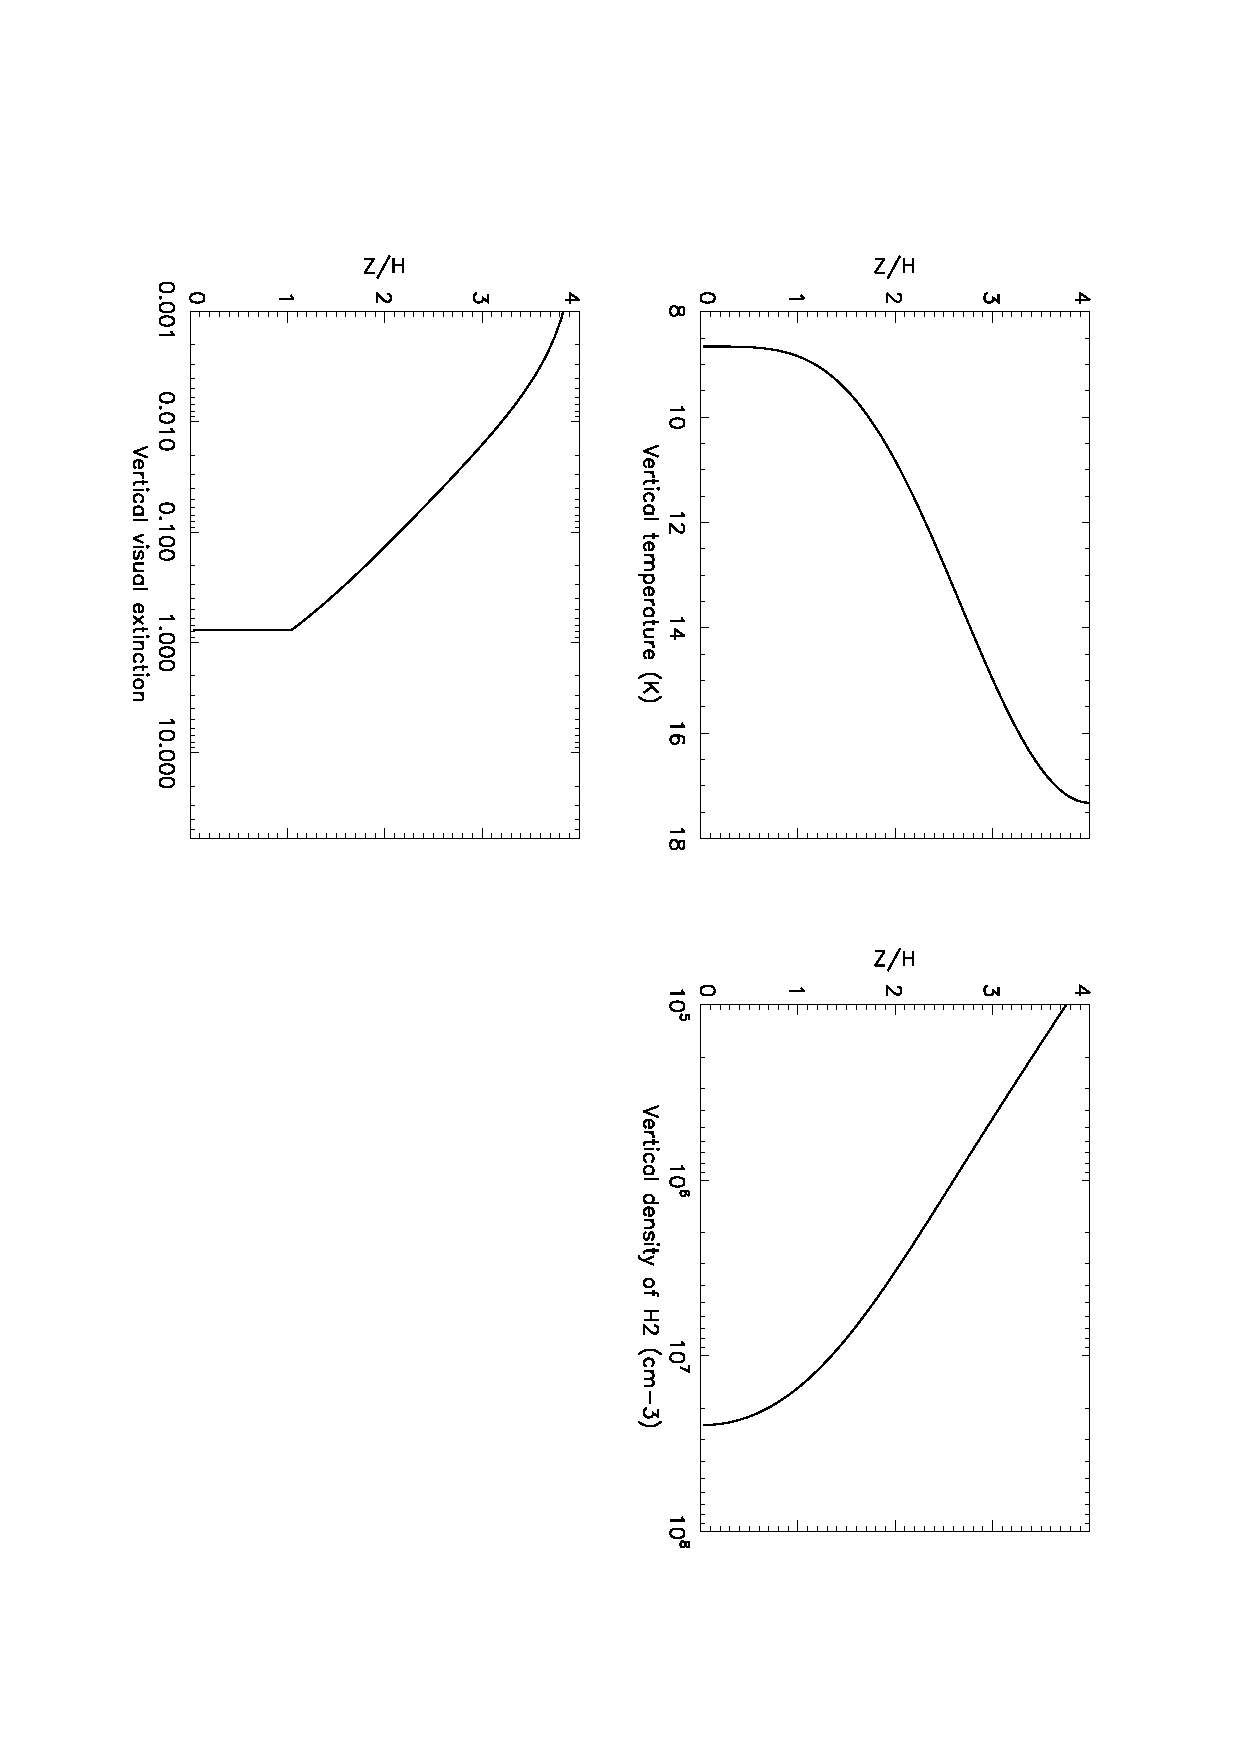
\includegraphics[angle=90,scale=.5]{disk_two_size.pdf}
\caption{Physical model computed for two different layers of dust: small grains of $10^{-5}$ cm above Z/H=1 and big grains of $3\times 10^{-3}$ below. The dust-to-gas mass ratio is $10^{-3}$ above Z/H=1 and $1.9\times 10^{-2}$ below.}
\label{fig2}
\end{figure}


\section{References}
%\vspace{-0.4cm}

\noindent Pi�tu, V., Dutrey, A., \& Guilloteau, S. 2007, A\&A, 467, 163\\

\noindent Guilloteau, S. \& Dutrey, A. 1998, A\&A, 339, 467 \\

\noindent Guilloteau, S., Dutrey, A., Pi�tu, V., \& Boehler, Y. 2011, A\&A, 529, A105\\

\noindent Bergin, E., Calvet, N., Sitko, M. L., et al. 2004, ApJ, 614, L133\\

\noindent Herczeg, G. J., Wood, B.E., Linsky, J. L., Valenti, J. A., \& JohnsKrull, C. M. 2004, ApJ, 607, 369\\

\noindent Dutrey et al., 2014, nature , 514, 600\\

\noindent  Hersant et al., 2009, A\&A, 493, L49\\

\noindent  Andrews S.M et al.,  2012. ApJ, 744, 162\\

\noindent Qi C., Wilner D. J., Calvet N., Bourke T. L., Blake G. A., Hogerheijde M. R., Ho P. T. P., Bergin E., 2006, ApJL, 636, L157 \\

\noindent Mayer,  L.,  Lufkin,  G.,  Quinn,  T.,  \&  Wadsley,  J.  2007, ApJL, 661, L77 \\

\end{document}